\documentclass{article}

% if you need to pass options to natbib, use, e.g.:
% \PassOptionsToPackage{numbers, compress}{natbib}
% before loading nips_2016
%
% to avoid loading the natbib package, add option nonatbib:
% \usepackage[nonatbib]{nips_2016}

\usepackage[final]{nips_2016}

% to compile a camera-ready version, add the [final] option, e.g.:
% \usepackage[final]{nips_2016}

\usepackage[utf8]{inputenc} % allow utf-8 input
\usepackage[T1]{fontenc}    % use 8-bit T1 fonts
\usepackage{hyperref}       % hyperlinks
\usepackage{url}            % simple URL typesetting
\usepackage{booktabs}       % professional-quality tables
\usepackage{amsfonts}       % blackboard math symbols
\usepackage{nicefrac}       % compact symbols for 1/2, etc.
\usepackage{microtype}      % microtypography
\usepackage{graphicx}
\usepackage{subfigure}

\title{Project 2 Part 2: Using Recurrent Neural Networks for Regression}

% The \author macro works with any number of authors. There are two
% commands used to separate the names and addresses of multiple
% authors: \And and \AND.
%
% Using \And between authors leaves it to LaTeX to determine where to
% break the lines. Using \AND forces a line break at that point. So,
% if LaTeX puts 3 of 4 authors names on the first line, and the last
% on the second line, try using \AND instead of \And before the third
% author name.

\author{
  Marcus ~Brenscheidt \\
  Heinrich Heine University\\
  \texttt{marcus.brenscheidt@uni-duesseldorf.de} \\
  %% examples of more authors
  \And
  Bastian Berndt \\
  Heinrich Heine University\\
  \texttt{bastian.berndt@uni-duesseldorf.de} \\
  \And
  Tobias Uelwer \\
  Heinrich Heine University\\
  \texttt{tobias.uelwer@uni-duesseldorf.de} \\
  %% \AND
  %% Coauthor \\
  %% Affiliation \\
  %% Address \\
  %% \texttt{email} \\
  %% \And
  %% Coauthor \\
  %% Affiliation \\
  %% Address \\
  %% \texttt{email} \\
  %% \And
  %% Coauthor \\
  %% Affiliation \\
  %% Address \\
  %% \texttt{email} \\
}

\begin{document}
%\nipsfinalcopy %is no longer used

\maketitle

\begin{abstract}
  This paper will show Recurrent Neural Networks (RNNs) used for regression on real world time series data. We will apply it to two different examples. 
\end{abstract}

\section{Introduction to the data and RNNs}
Both datasets will be split into training and test data, with the test dater always beeing the last 10\% of the data.
\subsection{Dataset 1}
The first dataset is a simple time series consisting of 1000 data points evenly distributed over [0,1] as $x$ and their corresponding functionvalues as $y$.

\subsection{Dataset 2}
The second dataset is a real world time series. It contains over 2800 samples, each representing the monthly mean relative number of sunspots. They range from the year of 1749 to 1983. Sunspots are spots on the sun, that seem darker than their sourroundings due to contrast. The data was collecting at the Swiss Federal Observation, Zurich till 1960 and at the Tokyo Astronomical Observatory afterwards. We renamed the columns to $x$ and $y$, so we could easily apply the code from the first dataset. $x$ cooresponds to the year and month (as float like 1949.33333), while $y$ displays the amount of sunspots.
\begin{figure}[h]
\centering
\subfigure{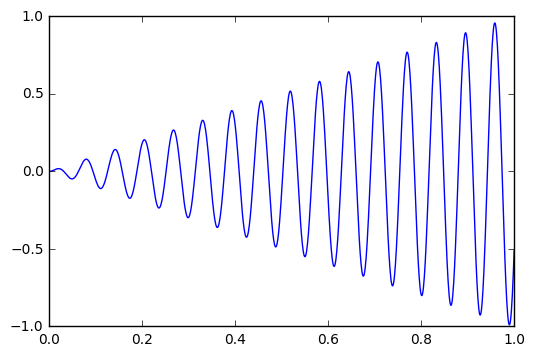
\includegraphics[width=0.45\textwidth]{images/xsinx.png}}
\subfigure{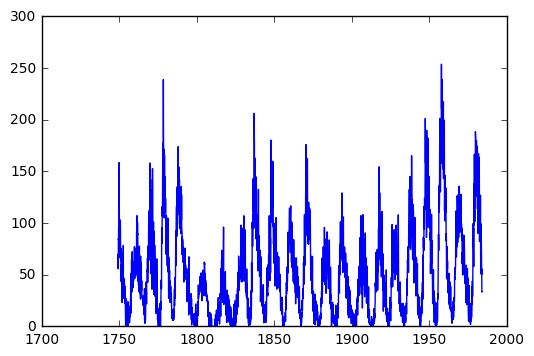
\includegraphics[width=0.45\textwidth]{images/sunspots.png}}
\caption{Left: project02 task2; Right: sunspots}
\end{figure}
\newpage
\subsection{On RNNs}
Recurrent Neural Networks are networks making use of sequential information by working in timesteps. We assume that inputs are dependent on previous ones, like the next word in a sentence depends on the ones before it. The main architecture used is the LSTM (Long Short-Term Memory). It consists of multiple stacked LSTM cells, each using information from previous cells to compute its own output and hand it to the next one, such that information is prolonged in the network. Additionally to that there is a cell state, which chains through all LSTM cells, each cell being able to add or remove information from the cell state. This way even longterm dependecies can be learned by the network.

\section{Architecture and Hyperparameters}
This section has already been subject in the previous report and will be done shorter here.
\subsection{Architecture}
The architecture is pretty simple. We basically use only LSTM cells on both datasets, even though we have the possibily to add dense layers at the end of the architecture, because we found they don't really give any additional accuracy. For the number of stacked LSTM cells we chose 20 for the first one and 150 for the second one, resembling the complexity of the given dataset. Adding to many cells leads to overfitting, so we rather chose less. As optimizer we use the Adamoptimizer and as loss the Mean Squared Error. Given this information our architecures were pretty straight forward and dont really need any special visualization.
\subsection{Effect of Iteration Count}
As long as we didn't converge, more itearations means we get closer to the desired minimum of the loss function. We found that 5000 training steps were fine for the datasets.

\subsection{Effect of Timesteps}
As timesteps we consider the number of datapoints we are able to look back at. This behaves similar to the number of stacked cells, making this too high might make us look at data, that is mostly independent from what we're looking at right now, while choosing it to low, removes valuable information. Another important aspect is the increase in computation time. Obviously looking at more data takes us longer to train the network. We choose 10 for the first and 100 for the second dataset.
\newpage
\section{Training and Performance}
\subsection{Training}
The training went basically the same as for the models of the first project. This time we decided to proceed in trainingsteps instead of epochs. One trainingstep is considered as shoving one batch of data through the model and optimizing the parameters on that one. By defining the model, giving an optimizer, a costfunction and explaining how to do prediction, we give tensorflow everything it needs to run its session and optimize the parameters. We track the amount of trainingsteps proceeded through and give some error each time we finish the complete trainingset, which is a simple way to babysit the trainingprocess. When the training is finished we shove the testdata through the network and then return the predicted values.
\subsection{Dataset 1}
On the first dataset we achieved mean squared errors of around 0.000050 on the test data and <0.000001 on the training data. The plot [Figure \ref{results}] below shows how close we got with just few seconds of training time
\subsection{Dataset 2}
The second dataset was way more complex, than the first one. It was hard to get really accurate predictions, but the setup we used, was showing somewhat of a smoothened version of the original [Figure \ref{results}]
\begin{figure}[h]
\centering
\subfigure{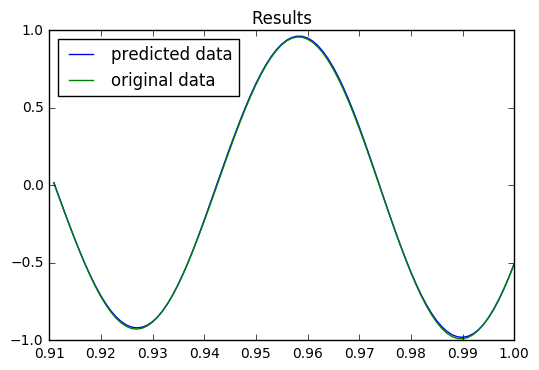
\includegraphics[width=0.45\textwidth]{images/test1.png}}
\subfigure{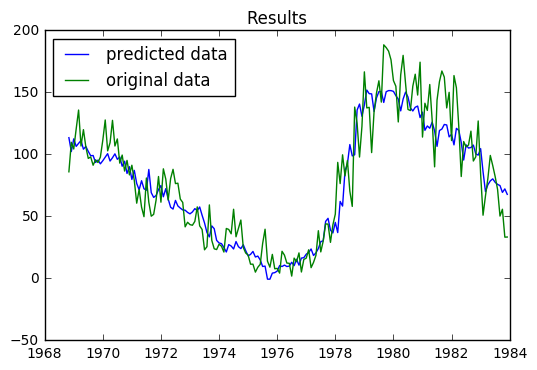
\includegraphics[width=0.45\textwidth]{images/test2.png}}
\caption{Left: results on the testdata of first dataset; Right: results on testdata of second dataset}
\label{results}
\end{figure}

\end{document}
